\begin{frame}
	\frametitle{Etapas para programação}
	\begin{figure}
		\centering
		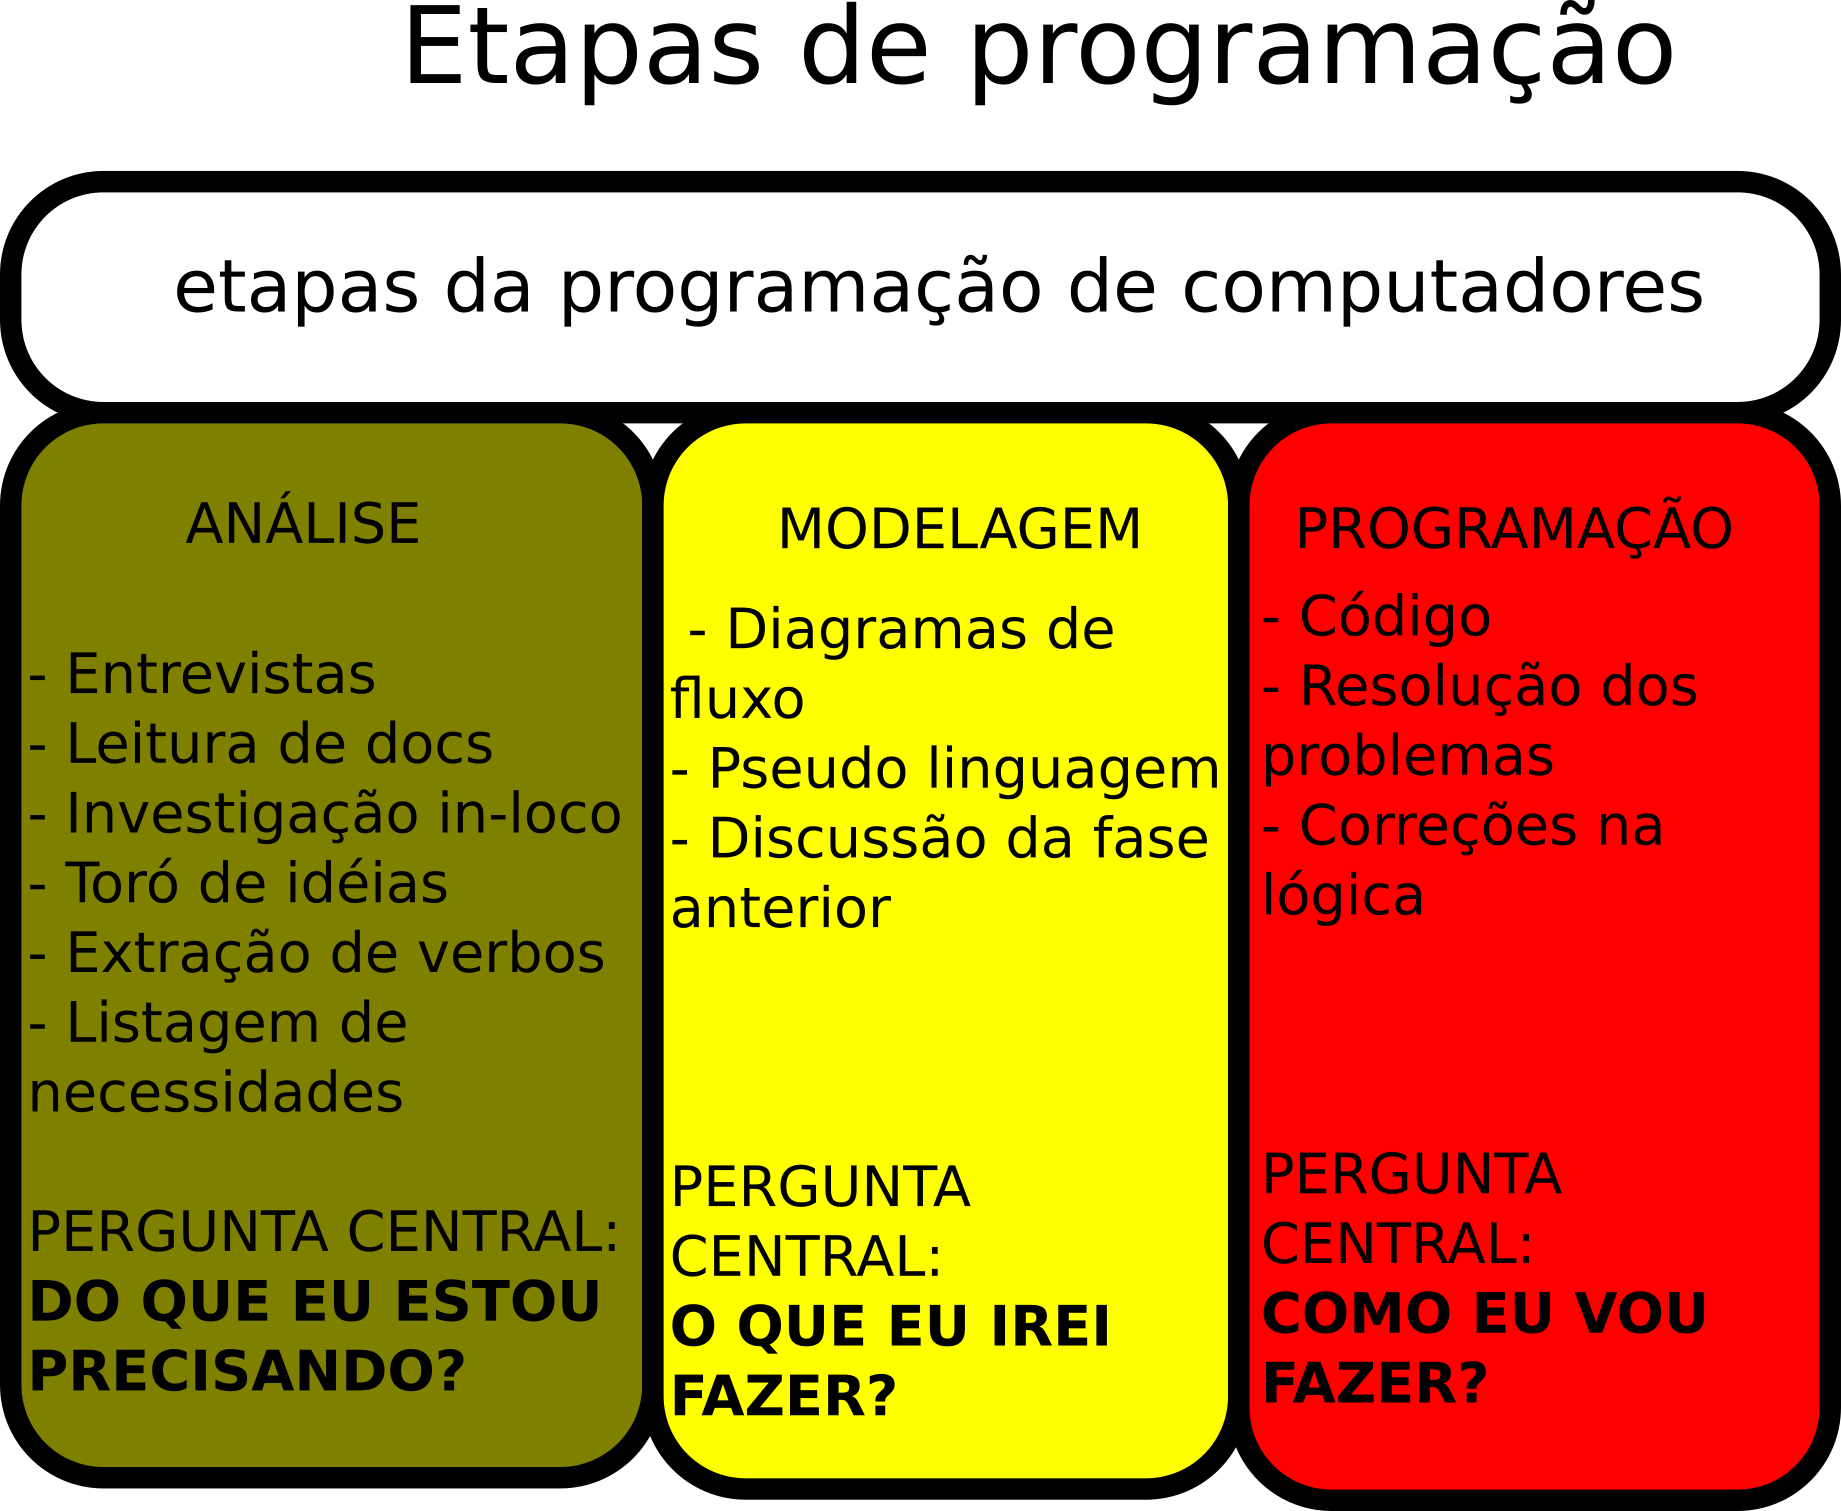
\includegraphics[width=0.6\linewidth]{images/etapasDeProgramacao}
		\caption{Etapas de programação}
		\label{fig:etapasdeprogramacao}
	\end{figure}
\end{frame}

\begin{frame}
	\frametitle{Etapas para programação}
	\begin{itemize}
		\item Entendimento das entradas e saídas.
		\item Definir estrutura de dados.
		\item Implementação.
		\item Demonstrar que funciona.
	\end{itemize}
\end{frame}


